\documentclass[11pt, oneside]{article}   	% use "amsart" instead of "article" for AMSLaTeX format
\usepackage{geometry}                		% See geometry.pdf to learn the layout options. There are lots.
\geometry{letterpaper}                   		% ... or a4paper or a5paper or ... 
%\geometry{landscape}                		% Activate for for rotated page geometry
\usepackage[parfill]{parskip}    			% Activate to begin paragraphs with an empty line rather than an indent
\usepackage{graphicx}				% Use pdf, png, jpg, or eps§ with pdflatex; use eps in DVI mode
								% TeX will automatically convert eps --> pdf in pdflatex	
\usepackage{amssymb}
\usepackage{amsmath}
\usepackage{listings}
\usepackage{color}

\date{}							% Activate to display a given date or no date

\newcommand{\tab} {\hspace*{2em}}
\newcommand{\stab} {\hspace*{.75em}}

\definecolor{codegreen}{rgb}{0,0.6,0}
\definecolor{codepurple}{rgb}{0.58,0,0.82}
\definecolor{codeblue}{rgb}{0,0,0.6}
\definecolor{codeorange}{rgb}{1,0.25,0}
\definecolor{backcolour}{rgb}{0.97,0.97,0.95}

\lstdefinestyle{gitlog}{
  backgroundcolor=\color{backcolour},
  breakatwhitespace=false, 
  breaklines=true,    
  keepspaces=true
  basicstyle=\ttfamily
  keyworkdstyle=\ttfamily
  commentstyle=\ttfamily
  identiferstyle=\ttfamily
  stringstyle=\ttfamily
  numbers=left,                    
  numbersep=5pt,  
  escapechar=/
  escapechar=_
  escapechar=\
  escapechar='
  escapechar=,
}

\lstdefinestyle{customc}{
  backgroundcolor=\color{backcolour},   
  keywordstyle=\bfseries\color{codegreen},
  commentstyle=\itshape\color{codepurple},
  identifierstyle=\color{codeblue},
  stringstyle=\color{codeorange},
  basicstyle=\footnotesize,
  breakatwhitespace=false,         
  breaklines=true,                 
  captionpos=b,                    
  keepspaces=true,                 
  numbers=left,                    
  numbersep=5pt,                  
  showspaces=false,                
  showstringspaces=false,
  showtabs=false,                  
  tabsize=2
}

\begin{document}

\begin{center}
\LARGE
Stitch Language Final Reportd\\[2em]
\Large 
Daniel Cole (System Architect), Megan Skrypek (Tester), Rashedul Haydar (Manager), Tim Waterman (Language Guru)\\
\large dhc2131, ms4985, rh2712, tbw2105\\[2em]
\normalsize
December 22, 2015\\[3em]
\end{center}

\newpage

\LARGE\textbf{Introduction}\\[2em]
\normalsize
Most "modern" programming languages trace their origins back decades to before the advent of cheap, general purpose multicore CPUs.  They were designed for a distinctly mono-threaded environment.  While libraries and enhancements to mainstay languages such as C/C++ and Java have added multithreading capabilities, it remains in many ways bolted on kludge.  While newer frameworks such as Node.js provide more integral support for asynchronous operations, they lack the depth of support and power of a fully compiled language.  With Stitch, we aim to build a language that has the power and flexibility of a fully compiled C style language, while having native threading support for modern multithreaded applications.  Our goal is to create a translator from Stitch to C.\\[.5em]
Stitch is inspired by C, which has a very well known syntax, and has been one of the most widely used languages since it was released over forty years ago.  Stitch is a general purpose language that supports all standard mathematical and logical operations.  Like C, Stitch is strongly typed, and whitespace does not matter.  In addition to the standard C primitive types (\verb|int, double, char|, etc.)\\[.5em]
Stitch is able to provide an easy to use, clear paradigm for multithreaded operations by strictly limiting when and how they can be invoked.  This is done through the \verb|stitch| loop.  The body of this loop is automatically split into multiple threads, and the program will not continue until all threads have returned.  Using a simple loop paradigm, similar to well know control structures like \verb|while| and \verb|for| loops, allows for an easy learning curve, and clear easy to read code.  It also allows the complier to easily see what code needs to be run in a threaded manner, and to efficiently generate the threaded code.\\[.5em]
The underlying method by which Stitch runs multithreaded code is C's \verb|pthread| library.  The Stitch complier will wrap the body of the \verb|stitch| loop in a function.  This function will be executed in parallel using \verb|pthreads|.  Variable scoping inside the threads is also handled by the complier.  Each threads is passed a C \verb|struct| that contains all non-local variables needed by the block of code that is being multithreaded.  This prevents clobbering issues without needing to resort to \verb|mutex| locks.  The only exceptions to this rule are accumulators, which are very limited in scope, and arrays, which can be sliced and piecewise accessed by different threads concurrently.   

\newpage

\LARGE\textbf{Language Tutorial}\\[2em]
\normalsize

\newpage

\LARGE\textbf{Language Reference Manual}\\[2em]
\normalsize

\newpage

\LARGE\textbf{Project Plan}\\[2em]
\normalsize

\Large\textbf{Planning}\\[1em]
\normalsize
We arranged weekly meetings with our language advisor Professor Edwards to discuss progress and issues that we countered. The immediate feedbacks we received from him were extremely helpful in the development of the language, especially when we were heading in the wrong directions. We had weekly meetings as well where all of us got together and worked on the project. During the meetings we split up the work, often two people working together on the same thing. Initially this worked really well since all of us were new with OCaml. Later, we divided up the work on an individual level such as implementing some functionality or writing some specific tests.\\[3em]
\Large\textbf{Style Guide}\\[1em]
\normalsize
While programming our compiler we tried to follow these general guidelines:
\begin{itemize}
  \item Ocaml style guidelines, such as indentation and formatting
  \item Tried to keep lines limited to 80 characters, if this wasn?t possible due to unreadability, then we used 120 characters as the hard limit.
  \item Unlike Ocaml, we named variables in all lowercase and used underscores as a delimiter
  \item Used 4-space indentation for each program 
\end{itemize}
\newpage
\Large\textbf{Project Timeline}\\[0em]
\normalsize
\tab\begin{description}
  \item[September 30] Proposal submitted
  \item[October 26] LRM submitted, scanner and parser with 1 shift/reduce error
  \item[November 16] Working scanner, parser, ast without arrays/stitch loops, \\[.5em]'Hello, Word' works
  \item[November 30] Finished semantic analyzer and cast
  \item[December 8] Finished c code generator with arrays added
  \item[December 14] Stitch loops working 
  \item[December 21] Final Presentation
  \item[December 22] Code cleanup and Final Report submitted 
\end{description}
\tab\\[3em]
\Large\textbf{Team Roles and Responsibilities}\\[1em]
\normalsize
\tab\begin{tabular}{l c l}
Rashedul Haydar & - & Manager\\
Tim Waterman & - & Language Guru\\
Dan Cole & - & System Architect\\
Megan Skrypek & - & Tester\\
\end{tabular}\\

While we had assigned roles, the responsibilities became much more fluid as the project progressed. During the initial planning phase we all discussed the structure and components of the language. Later on, we also worked together on the semantic analyzer, C generator, and the variety of tests used for the test suite.
\newpage
\Large\textbf{Software Development Environment}\\[1em]
\normalsize
\begin{itemize}
  \item Version Control
  \begin{itemize}
    \item Git
  \end{itemize}
  \item Languages
  \begin{itemize}
    \item OCaml (4.02.3) for parser, scanner, ast, semantic analysis
    \item GCC for compiling generated C code
    \item bash for test suite and singer
    \item Python (2.7.5) for image curve generator
    \item \LaTeX\ for reports and documentation
  \end{itemize}
  \item Text Editors 
    \begin{itemize}
    \item VIM
    \item Sublime
    \end{itemize}
\end{itemize}

\newpage
\Large\textbf{Project Log}\\[1em]
\normalsize
\lstinputlisting[style=gitlog]{commits.txt}

\newpage
\LARGE\textbf{Architectural Design}\\[2em]
\normalsize
\Large\textbf{Block Diagram}\\[1em]
\normalsize
\centerline{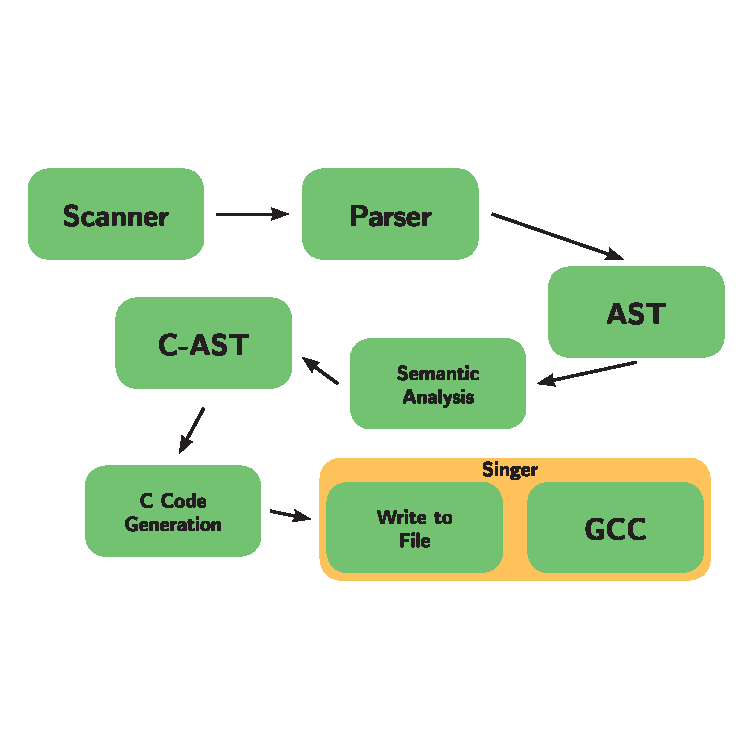
\includegraphics[scale=1.2]{block.pdf}}

\newpage
\Large\textbf{Interface Description}\\[1em]
\normalsize
\begin{tabular}{ l p{12cm} }
Scanner\\\verb|stch_scanner.mll| & The scanner is written in OCamlLex.  It takes input from the source file, and tokenizes it into keywords, identifiers, and literals.  It scans over and removes both single line and multi-line comments, as well as all whitespace not in string literals.  Any token that is not a keyword, or does not meet the criteria for an identifier or literal will throw a scanner error.\\[.5em]
Parser/AST\\ \verb|stch_parser.mly|\\\verb|stch_ast.ml| & The parser is written in OCamlYacc.  It takes the tokens from the scanner, and using the grammar defined in the parser and the datatypes defined in the AST, generates an abstract syntax tree.  The rules in the parser insure that code that passes this step is syntactically correct, although not necessarily semantically correct.  Any error at this stage will throw a syntax error.  The AST file also contains pretty printing functions for all datatypes defined therin.\\[.5em]
Semantic Checking/CAST\\ \verb|stch_ast.mll|\\\verb|stch_semantic.ml|\\\verb|stch.cast.mli| & Stitch first runs the AST through the semantic analyzer.  This pass insures that the code is semantically valid.  The output of the semantic analyzer is another AST, a C language AST.  The major difference here is that the CAST carries with it a Stitch Environment, which has, most importantly, a list of declared functions, and a symbol table, which contains all declared identifiers and their type.  Stitches symbol table also contains information on the expression that the identifier references, which is used in the C code generation to build pthread related code.\\[.5em]
\end{tabular}
\newpage
\begin{tabular}{ l p{12cm} }
Code Generation\\\verb|c_generator.ml| & The CAST, which as already been semantically analyzed is now pretty printed.  The bulk of the work to add multithreading is done here.  The C generator performs multiple passes on the CAST.  First any non-\verb|main| functions are printed.  Then any \verb|stitch| loops are analyzed, and their statements are turned into a function.  Finally, \verb|main| is printed.  This insures proper scoping of functions, and that all functions declared before main can be called in any Stitch block.  To convert \verb|stitch| loops to multithreaded \verb|pthread| code, the C generator first takes the body of the loop and transforms it into a function.  The generator also builds a custom \verb|struct| for each \verb|stitch| loop, that contains all in-scope, non-local variables that the loop will need access too.  It then generates the \verb|pthread| specific code, as well as a \verb|for| loop that creates and runs the threads.  The function containing the code body, as well as the structure containing all needed variables is passed into the \verb|pthread|.
\end{tabular}
\newpage


\LARGE\textbf{Test Plan}\\[2em]
\normalsize

\Large\textbf{GCD}\\[1em]
\normalsize
\lstinputlisting[language=C, style=customc, caption=Stitch]{gcd.stch}
\newpage
\Large\textbf{GCD}\\[1em]
\normalsize
\lstinputlisting[language=C, style=customc, caption=C]{gcd.stch.c}
\newpage
\Large\textbf{Stitch loop Matrix Multiplication}\\[1em]
\normalsize
\lstinputlisting[language=C, style=customc, caption=Stitch]{matrixstitch.stch}
\newpage
\Large\textbf{Stitch loop Matrix Multiplication}\\[1em]
\normalsize
\lstinputlisting[language=C, style=customc, caption=C]{matrixstitch.stch.c}
\newpage
\Large\textbf{Test Suite Log}\\[1em]
\normalsize
Full test code supplied in appendix\\
\lstinputlisting{Dec22_175129_test_log.txt}
\newpage
\Large\textbf{Test Description}\\[1em]
\normalsize
We started with a basic hello world program and then started adding cases such as basic arithmetic, comparison and logical operations, conditionals, comments, functions etc. Once we were able to get the basics passing the test suite, we moved on to semantic checking, arrays (1D and 2D), file I/O, and stitch loops. We added negative tests for certain features for a more comprehensive testing suite.\\

Positive Tests\\
\begin{itemize}
\item Basic arithmetic
\item Comparison ops
\item Logical ops, negate
\item Conditional statements
\begin{itemize}
\item Nested variable declarations
\item Nested conditional statements
\end{itemize}
\item Comments- single and multiple lines
\item Functions- single, multiple, gcd
\item Break, exit
\item Type checking
\item 1D arrays, initializing and assigning
\item 2D arrays (matrices), initializing and assigning
\item File I/O
\item Stitch Loops
\item Matrix multiplication
\item Escaped characters
\item Accumulators
\end{itemize}

\newpage

Negative Tests\\
\begin{itemize}
\item Arithmetic with mismatched types
\item Type checking with void
\item Negate with floats, chars
\item Global variables
\item Comments
\item Functions
\begin{itemize}
\item Initializing variables as arguments
\item No return type
\item Declaring functions inside functions
\item Calling undeclared functions
\end{itemize}
\item Arrays
\begin{itemize}
\item Initializing, accessing, size parameter as expression
\end{itemize}
\item Matrices
\begin{itemize}
\item Initializing, accessing
\end{itemize}
\item Print/error with wrong type
\item File I/O
\item Invalid conditionals
\item Stitch Loops
\begin{itemize}
\item Undeclared iterator variable
\item No curly braces around statement block
\end{itemize}
\end{itemize}
\newpage

\Large\textbf{Test Automation}\\[1em]
\normalsize
The test suite stch\_testSuite.sh first makes the compiler, then iterates through each test in the positive tests folder, calling the tool chain ?Singer?. ?Singer? runs the compiler on the test program, generating the c code, and compiling the c program with the appropriate runtime headers and c libraries. The test suite then checks if the file compiled, and prints the appropriate response to the screen and the log. It compares the difference between the output generated by the executable and the expected output, and prints the result to the screen and to the log. The negative tests are iterated through in a similar way, however the test only passes if the compilation fails. Finally, the test suite cleans up all the target programs, generated output, and executables.

Tests were added by all members of our team as they were needed. The test script is located in the appendix.


\newpage
\LARGE\textbf{Lessons Lerned}\\[2em]
\normalsize

\Large\textbf{Rashedul Haydar}\\[1em]
\normalsize
\tab For a semester long project it?s very important to try to get at least parts of the project done each week. Thankfully, we planned enough to have progress each week on the project. Having the weekly meetings with our advisor really pushed us to get something done every week. Even with the incremental progress, the last two weeks of the project was still crazy. 

\newpage
\Large\textbf{Megan Skrypek}\\[1em]
\normalsize
\tab I learned how important planning and communication is in tackling a large project like this. Having weekly meetings to work on components of the project as well as discuss future plans really helped us manage our time. Working on key components as a team really helped every member understanding the overall flow of the project, instead of only handling individual components. Some advice for future teams would be to start as early as possible, if you get stuck in the beginning it is very difficult to finish on time since each piece of the compiler builds on one another.

\newpage
\Large\textbf{Daniel Cole}\\[1em]
\normalsize
\tab First and foremost, this was an amazing learning opportunity.  Beyond learning the PLT related topics of complier design, I learned group management, how to work on large scale, long term projects, how to integrate code written by multiple people, and how to partition tasks.  One of the big challenges was the long scale of the project.  Keeping everything moving, and everyone motivated when the deadline was far away was not always easy.  The periodic milestones, as well as the weekly checkins help immensely.\\[.5em]
\tab Because so much of our language focused on the C code generation, when we got to that point, (from the end of November on), it became much harder to split up the work, as most work at this point was dependent on previous work, and had to be completed in sequence.  For instance, matrices needed arrays done first, and the Stitch loop bodies needed the Stitch functions done first.  Along with other classwork, this was the biggest issue we had with balancing the workload.\\[.5em]
\tab I'd also like to confirm pretty much everything you said at the beginning of the semester, especially regarding OCaml.  It wasn't until around the time I finished up the semantic analyzer that I fully appreciated why you had us work in this language.  While it won't be my first choice for most projects going forwards, for this type of thing, it is 100\% the best language I can imagine.

\newpage
\Large\textbf{Tim Waterman}\\[1em]
\normalsize
\newpage

\newpage
\LARGE\textbf{Code}\\[2em]
\normalsize

\end{document}
